
\begin{figure}[H]
   \centering
   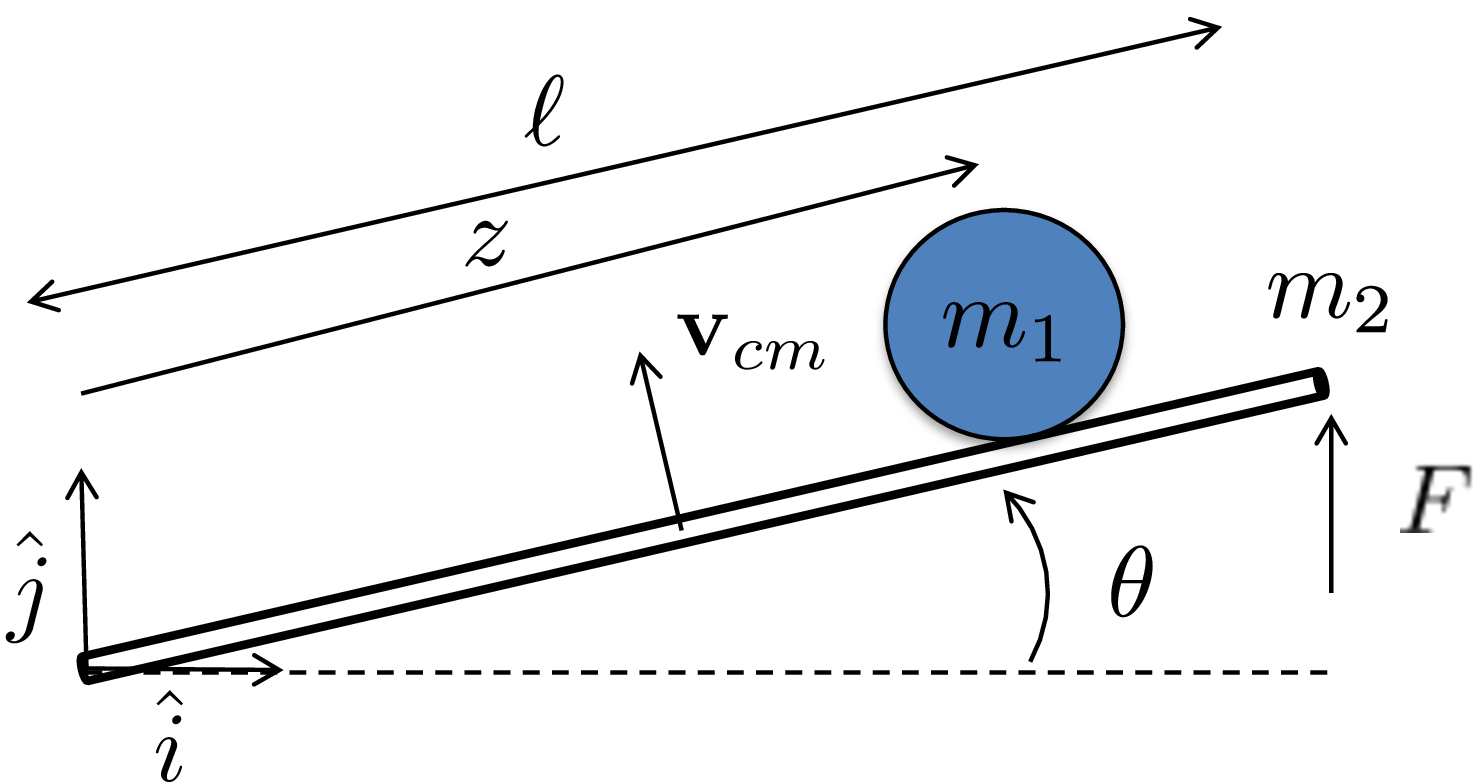
\includegraphics[width=0.5\textwidth]{6_design_studies/figures/hw_ballbeam_kinetic_energy} 
   \caption{Computing the kinetic energy for the ball on beam system.}
   \label{fig:hw_ballbeam_kinetic_energy}
\end{figure}


Define the inertial coordinate frame as in Figure~\ref{fig:hw_ballbeam_kinetic_energy}, with $\hat{k}$ out of the page.  

Since there are two masses, the total kinetic energy of the system is given by
\[
K = \frac{1}{2}m_{ball} \mathbf{v}^{\top}_{ball} \mathbf{v}_{ball} + \frac{1}{2}\boldsymbol{\omega}_{ball}^{\top}J_{ball}\boldsymbol{\omega}_{ball} 
+ \frac{1}{2}m_{beam} \mathbf{v}^{\top}_{beam} \mathbf{v}_{beam} + \frac{1}{2}\boldsymbol{\omega}_{beam}^{\top}J_{beam}\boldsymbol{\omega}_{beam}.
\]
We will assume that the ball moves without rolling and therefore that $\boldsymbol{\omega}_{ball}=0$.

The horizontal position of the ball $m$ is given by 
\[
\mathbf{p}_{ball} = \begin{pmatrix} z(t)\cos\theta(t) \\ z(t)\sin\theta(t) \\ 0 \end{pmatrix}.
\]
Similarly, the position of the center of mass of the beam is given by
\[
\mathbf{p}_{beam} = \begin{pmatrix} \frac{\ell}{2}\cos\theta(t) \\ \frac{\ell}{2}\sin\theta(t) \\ 0 \end{pmatrix}.
\]

Differentiating we obtain
\begin{align*}
\mathbf{v}_{ball} &= \begin{pmatrix} \dot{z}\cos\theta - z\dot{\theta}\sin\theta \\ \dot{z}\sin\theta + z\dot{\theta}\cos\theta \\ 0 \end{pmatrix} \\
\mathbf{v}_{beam} &= \begin{pmatrix} -\frac{\ell}{2}\dot{\theta}\sin\theta \\ \frac{\ell}{2}\dot{\theta}\cos\theta \\ 0 \end{pmatrix}.
\end{align*}

The angular velocity of the beam is given by
\[
\boldsymbol{\omega}_{beam} = \begin{pmatrix} 0 \\ 0 \\ \dot{\theta} \end{pmatrix}.
\]
Therefore, the kinetic energy is given by
\begin{align*}
K &= \frac{1}{2}m_{1} \left[ (\dot{z}\cos\theta - z\dot{\theta}\sin\theta)^2 + (\dot{z}\sin\theta + z\dot{\theta}\cos\theta)^2 \right] 
\\ &\qquad
	+ \frac{1}{2}m_{2} \left[ (-\frac{\ell}{2}\dot{\theta}\sin\theta)^2 + (\frac{\ell}{2}\dot{\theta}\cos\theta)^2 \right]
	+ \frac{1}{2} J_z \dot{\theta}^2,
\end{align*}
where $J_z$ is the $(3,3)$ element of the inertia matrix $J_{beam}$.  Modeling the beam as a thin rod we have
\[
J_z = \frac{m_2\ell^2}{12}.
\]
Therefore
\begin{align*}
K &= \frac{1}{2}m_{1} \left[ \dot{z}^2\cos^2\theta - 2z\dot{z}\dot{\theta}\sin\theta\cos\theta + z^2\dot{\theta}^2\sin^2\theta + \dot{z}^2\sin^2\theta + 2z\dot{z}\dot{\theta}\sin\theta\cos\theta + z^2\dot{\theta}^2\cos^2\theta \right] 
\\ &\qquad
	+ \frac{1}{2}m_{2} \left[ \frac{\ell^2}{4}\dot{\theta}^2\sin^2\theta + \frac{\ell^2}{4}\dot{\theta}^2\cos^2\theta \right]
	+ \frac{1}{2} J_z \dot{\theta}^2, \\
	&= \frac{1}{2}m_{1} \left( \dot{z}^2 + z^2\dot{\theta}^2 \right) 
	+ \frac{1}{2} \frac{m_{2}\ell^2}{3} \dot{\theta}^2 \\
	&= \frac{1}{2}m_{1} \dot{z}^2 + \frac{1}{2} \left(\frac{m_{2}\ell^2}{3} + m_1 z^2\right) \dot{\theta}^2.
\end{align*}






